\section{Data Mining through RAVEN}
\label{sec:DMraven}

Data mining is the computational process of discovering patterns in large data sets (``big data'') involving methods at the intersection of artificial intelligence, machine learning, statistics, and database systems. The overall goal of the data mining process is to extract information from a data set and transform it into an understandable structure for further use.
\\RAVEN has support of several different data mining algorithms,
such as:
\begin{enumerate}
  \item \textit{Hierarchical methodologies}
  \item \textit{K-Means}
  \item \textit{Mean-Shift}, etc.
\end{enumerate}

The goals of this section are about learning how to:
 \begin{enumerate}
   \item Set up a sampling strategy to apply clustering algorithms, perturbing a driven code
  \item Analyze the data using clustering algorithms.
\end{enumerate}
To accomplish these tasks, the following RAVEN \textbf{Entities} (XML blocks in the input files) need to be defined:
\begin{enumerate}
   \item \textbf{\textit{RunInfo}}:
     \xmlExample{framework/user_guide/DataMining/dataMiningAnalysis.xml}{RunInfo}
   The \textit{RunInfo} \textbf{Entity} is intended  to set up the analysis sequence that
   needs to be performed. The number of steps specified in (\xmlNode{Sequence}) are sequentially run
   using the number of processors assigned in (\xmlNode{batchSize}).
   \\In the first step, the original physical model is going to be sampled.
   The obtained results are going to be analyzed with data mining
   algorithms.
   \item \textbf{\textit{Models}}:
     \xmlExample{framework/user_guide/DataMining/dataMiningAnalysis.xml}{Models}
 The goal of this example is to show how the
 data mining algorithms in RAVEN can be useful to analyze large data set.
 \\In addition to an External model, two Post-Processor models ($DataMining|cluster|KMeans$ and $DataMining|decomposition|PCA$) are specified. Note that the post-processing is performed on all the output FOMs used in this example ($r and t$).
   \item \textbf{\textit{Distributions}}:
     \xmlExample{framework/user_guide/DataMining/dataMiningAnalysis.xml}{Distributions}
  In the Distributions XML section, the stochastic model for the
  uncertainties are reported. In this case 2 distributions are defined:
  \begin{itemize}
    \item $vel\_dist \sim \mathbb{N}(30,5)$, used to model the uncertainties
    associated with  the \textit{velocity};
    \item  $angle\_dist \sim \mathbb{U}(5,85)$,  used to
    model the uncertainties associated with the \textit{angle}.
  \end{itemize}
   \item \textbf{\textit{Samplers}}:
     \xmlExample{framework/user_guide/DataMining/dataMiningAnalysis.xml}{Samplers}
  In order to obtain the data-set on which the data mining algorithms are going to be applied, a \textit{MonteCarlo} sampling approach is employed here.
   \item \textbf{\textit{DataObjects}}:
     \xmlExample{framework/user_guide/DataMining/dataMiningAnalysis.xml}{DataObjects}
  In this block, three \textit{DataObjects} are defined:
  1) PointSet named ``samples'' used to collect the final outcomes of
  the code,
  2) PointSet named ``dummyIN'' used as a placeholder for the \textit{Multirun} step,
  3) HistorySet named ``histories'' in which the full time responses of the
  variables $x,y,t$ are going to be stored.
 %figure samples
 \begin{figure}[h!]
  \centering
  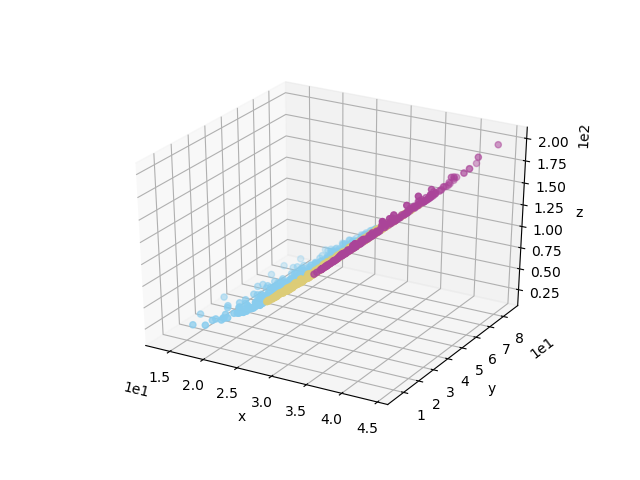
\includegraphics[scale=0.7]{../../tests/framework/user_guide/DataMining/gold/dataMiningAnalysis/1-PlotLabels_dataMining.png}
  \caption{K-means clustering on original dataset.}
  \label{fig:KmeanOrigData}
 \end{figure}
   \item \textbf{\textit{OutStreams}}:
     \xmlExample{framework/user_guide/DataMining/dataMiningAnalysis.xml}{OutStreams}
     This workflow uses one Print OutStream and three Plot OutStreams:
     \begin{itemize}
       \item ``samplesDump'', which writes the original sample set with the additional columns from the
         PostProcess steps,
       \item ``PlotKMeans1'', which plots the samples against the Figures of Merit with coloring according to the KMeans clustering,
       \item ``PlotLabels'', which plots the samples and colors them according to the KMeans clustering,
       \item ``PlotPCA1,'' which plots the surrogate principal component dimensions and their associated clustering.
     \end{itemize}
     Note that a special kind of plot, the ``dataMining'' \xmlNode{type}, has been implemented to simplify plotting complicated results using RAVEN, and is used in all three of the plots in this workflow.  Also note the use of the \xmlNode{range} block to define the data range of the plots created.
   \item \textbf{\textit{Steps}}:
     \xmlExample{framework/user_guide/DataMining/dataMiningAnalysis.xml}{Steps}

 %%%%%%%%%%%%%%%%%%%%%%%%%%%%%%%%%%%%%%%%%%%%%%%%%%%%%%%%%%
 %%%%%%%%%%%%%%%%%%%%%%%%%%%%%%%%%%%%%%%%%%%%%%%%%%%%%%%%%%
   Finally, all the previously defined \textbf{Entities} can be combined in
   the \xmlNode{Steps} block;
   3 \xmlNode{Steps} have been inputted:
   \begin{itemize}
     \item \xmlNode{MultiRun} named ``sample'', used to run the
     multiple
     instances of the driven code and
     collect the outputs in the two \textit{DataObjects}.The \xmlNode{Sampler} is inputted to communicate to the
     \textit{Step} that the driven code needs to
     be perturbed through the MonteCarlo sampling strategy;
     \item \xmlNode{PostProcess} named ``kmeans'', used
     to analyze the data obtained through the sampling strategy. In
     this step, a K-Means algorithm is going to be employed, plotting
     the clustering results;
     \textit{Step} that the driven code needs to
     be perturbed through the MonteCarlo sampling strategy;
     \item \xmlNode{PostProcess} named ``pca'', used
     to analyze the data obtained through the sampling strategy. In
     this Step, a PCA algorithm is going to be employed, plotting
     the decomposition results.
   \end{itemize}
\end{enumerate}
Figure~\ref{fig:KmeanOrigData} shows the clustering on the input space and the range, coloring according to the KMeans clustering,.
\\Figure~\ref{fig:KmeanProjected} shows the clustering on the range-angle and range-velocity plots respectively.
\\Figure~\ref{fig:PCAplot} shows the PCA decomposition on the data set.
%%%%%%%%%%%%%%%%%%%%%%%%%%%%%%%%%%%%%%%%%%%%%%%%%%%%%%%%%%
 %figure samples
 \begin{figure}[h!]
  \centering
  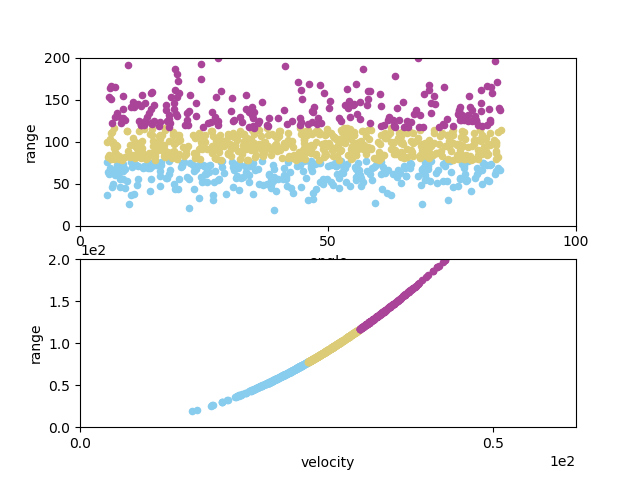
\includegraphics[scale=0.7]{../../tests/framework/user_guide/DataMining/gold/dataMiningAnalysis/1-PlotKMeans1_dataMining-dataMining.png}
  \caption{K-means clustering on projected parameters.}
  \label{fig:KmeanProjected}
 \end{figure}
 %%%%%%%%%%%%%%%%%%%%%%%%
 %%%%%%%%%%%%%%%%%%%%%%%%%%%%%%%%%%%%%%%%%%%%%%%%%%%%%%%%%%

 %%%%%%%%%%%%%%%%%%%%%%%%
  %%%%%%%%%%%%%%%%%%%%%%%%%%%%%%%%%%%%%%%%%%%%%%%%%%%%%%%%%%
 %figure samples
 \begin{figure}[h!]
  \centering
  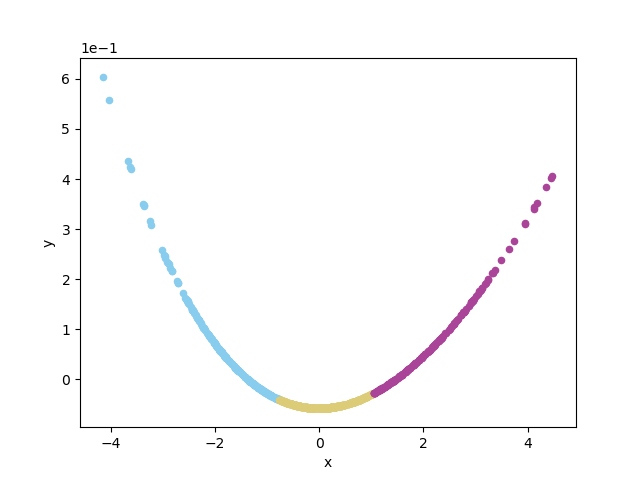
\includegraphics[scale=0.7]{../../tests/framework/user_guide/DataMining/gold/dataMiningAnalysis/1-PlotPCA1_dataMining.png}
  \caption{Principal Component Analysis.}
  \label{fig:PCAplot}
 \end{figure}
 %%%%%%%%%%%%%%%%%%%%%%%%

